\documentclass{article}
\usepackage{iclr2027_conference,times}
%%%%% NEW MATH DEFINITIONS %%%%%

\usepackage{amsmath,amsfonts,bm}

% Mark sections of captions for referring to divisions of figures
\newcommand{\figleft}{{\em (Left)}}
\newcommand{\figcenter}{{\em (Center)}}
\newcommand{\figright}{{\em (Right)}}
\newcommand{\figtop}{{\em (Top)}}
\newcommand{\figbottom}{{\em (Bottom)}}
\newcommand{\captiona}{{\em (a)}}
\newcommand{\captionb}{{\em (b)}}
\newcommand{\captionc}{{\em (c)}}
\newcommand{\captiond}{{\em (d)}}

% Highlight a newly defined term
\newcommand{\newterm}[1]{{\bf #1}}


% Figure reference, lower-case.
\def\figref#1{figure~\ref{#1}}
% Figure reference, capital. For start of sentence
\def\Figref#1{Figure~\ref{#1}}
\def\twofigref#1#2{figures \ref{#1} and \ref{#2}}
\def\quadfigref#1#2#3#4{figures \ref{#1}, \ref{#2}, \ref{#3} and \ref{#4}}
% Section reference, lower-case.
\def\secref#1{section~\ref{#1}}
% Section reference, capital.
\def\Secref#1{Section~\ref{#1}}
% Reference to two sections.
\def\twosecrefs#1#2{sections \ref{#1} and \ref{#2}}
% Reference to three sections.
\def\secrefs#1#2#3{sections \ref{#1}, \ref{#2} and \ref{#3}}
% Reference to an equation, lower-case.
\def\eqref#1{equation~\ref{#1}}
% Reference to an equation, upper case
\def\Eqref#1{Equation~\ref{#1}}
% A raw reference to an equation---avoid using if possible
\def\plaineqref#1{\ref{#1}}
% Reference to a chapter, lower-case.
\def\chapref#1{chapter~\ref{#1}}
% Reference to an equation, upper case.
\def\Chapref#1{Chapter~\ref{#1}}
% Reference to a range of chapters
\def\rangechapref#1#2{chapters\ref{#1}--\ref{#2}}
% Reference to an algorithm, lower-case.
\def\algref#1{algorithm~\ref{#1}}
% Reference to an algorithm, upper case.
\def\Algref#1{Algorithm~\ref{#1}}
\def\twoalgref#1#2{algorithms \ref{#1} and \ref{#2}}
\def\Twoalgref#1#2{Algorithms \ref{#1} and \ref{#2}}
% Reference to a part, lower case
\def\partref#1{part~\ref{#1}}
% Reference to a part, upper case
\def\Partref#1{Part~\ref{#1}}
\def\twopartref#1#2{parts \ref{#1} and \ref{#2}}

\def\ceil#1{\lceil #1 \rceil}
\def\floor#1{\lfloor #1 \rfloor}
\def\1{\bm{1}}
\newcommand{\train}{\mathcal{D}}
\newcommand{\valid}{\mathcal{D_{\mathrm{valid}}}}
\newcommand{\test}{\mathcal{D_{\mathrm{test}}}}

\def\eps{{\epsilon}}


% Random variables
\def\reta{{\textnormal{$\eta$}}}
\def\ra{{\textnormal{a}}}
\def\rb{{\textnormal{b}}}
\def\rc{{\textnormal{c}}}
\def\rd{{\textnormal{d}}}
\def\re{{\textnormal{e}}}
\def\rf{{\textnormal{f}}}
\def\rg{{\textnormal{g}}}
\def\rh{{\textnormal{h}}}
\def\ri{{\textnormal{i}}}
\def\rj{{\textnormal{j}}}
\def\rk{{\textnormal{k}}}
\def\rl{{\textnormal{l}}}
% rm is already a command, just don't name any random variables m
\def\rn{{\textnormal{n}}}
\def\ro{{\textnormal{o}}}
\def\rp{{\textnormal{p}}}
\def\rq{{\textnormal{q}}}
\def\rr{{\textnormal{r}}}
\def\rs{{\textnormal{s}}}
\def\rt{{\textnormal{t}}}
\def\ru{{\textnormal{u}}}
\def\rv{{\textnormal{v}}}
\def\rw{{\textnormal{w}}}
\def\rx{{\textnormal{x}}}
\def\ry{{\textnormal{y}}}
\def\rz{{\textnormal{z}}}

% Random vectors
\def\rvepsilon{{\mathbf{\epsilon}}}
\def\rvtheta{{\mathbf{\theta}}}
\def\rva{{\mathbf{a}}}
\def\rvb{{\mathbf{b}}}
\def\rvc{{\mathbf{c}}}
\def\rvd{{\mathbf{d}}}
\def\rve{{\mathbf{e}}}
\def\rvf{{\mathbf{f}}}
\def\rvg{{\mathbf{g}}}
\def\rvh{{\mathbf{h}}}
\def\rvu{{\mathbf{i}}}
\def\rvj{{\mathbf{j}}}
\def\rvk{{\mathbf{k}}}
\def\rvl{{\mathbf{l}}}
\def\rvm{{\mathbf{m}}}
\def\rvn{{\mathbf{n}}}
\def\rvo{{\mathbf{o}}}
\def\rvp{{\mathbf{p}}}
\def\rvq{{\mathbf{q}}}
\def\rvr{{\mathbf{r}}}
\def\rvs{{\mathbf{s}}}
\def\rvt{{\mathbf{t}}}
\def\rvu{{\mathbf{u}}}
\def\rvv{{\mathbf{v}}}
\def\rvw{{\mathbf{w}}}
\def\rvx{{\mathbf{x}}}
\def\rvy{{\mathbf{y}}}
\def\rvz{{\mathbf{z}}}

% Elements of random vectors
\def\erva{{\textnormal{a}}}
\def\ervb{{\textnormal{b}}}
\def\ervc{{\textnormal{c}}}
\def\ervd{{\textnormal{d}}}
\def\erve{{\textnormal{e}}}
\def\ervf{{\textnormal{f}}}
\def\ervg{{\textnormal{g}}}
\def\ervh{{\textnormal{h}}}
\def\ervi{{\textnormal{i}}}
\def\ervj{{\textnormal{j}}}
\def\ervk{{\textnormal{k}}}
\def\ervl{{\textnormal{l}}}
\def\ervm{{\textnormal{m}}}
\def\ervn{{\textnormal{n}}}
\def\ervo{{\textnormal{o}}}
\def\ervp{{\textnormal{p}}}
\def\ervq{{\textnormal{q}}}
\def\ervr{{\textnormal{r}}}
\def\ervs{{\textnormal{s}}}
\def\ervt{{\textnormal{t}}}
\def\ervu{{\textnormal{u}}}
\def\ervv{{\textnormal{v}}}
\def\ervw{{\textnormal{w}}}
\def\ervx{{\textnormal{x}}}
\def\ervy{{\textnormal{y}}}
\def\ervz{{\textnormal{z}}}

% Random matrices
\def\rmA{{\mathbf{A}}}
\def\rmB{{\mathbf{B}}}
\def\rmC{{\mathbf{C}}}
\def\rmD{{\mathbf{D}}}
\def\rmE{{\mathbf{E}}}
\def\rmF{{\mathbf{F}}}
\def\rmG{{\mathbf{G}}}
\def\rmH{{\mathbf{H}}}
\def\rmI{{\mathbf{I}}}
\def\rmJ{{\mathbf{J}}}
\def\rmK{{\mathbf{K}}}
\def\rmL{{\mathbf{L}}}
\def\rmM{{\mathbf{M}}}
\def\rmN{{\mathbf{N}}}
\def\rmO{{\mathbf{O}}}
\def\rmP{{\mathbf{P}}}
\def\rmQ{{\mathbf{Q}}}
\def\rmR{{\mathbf{R}}}
\def\rmS{{\mathbf{S}}}
\def\rmT{{\mathbf{T}}}
\def\rmU{{\mathbf{U}}}
\def\rmV{{\mathbf{V}}}
\def\rmW{{\mathbf{W}}}
\def\rmX{{\mathbf{X}}}
\def\rmY{{\mathbf{Y}}}
\def\rmZ{{\mathbf{Z}}}

% Elements of random matrices
\def\ermA{{\textnormal{A}}}
\def\ermB{{\textnormal{B}}}
\def\ermC{{\textnormal{C}}}
\def\ermD{{\textnormal{D}}}
\def\ermE{{\textnormal{E}}}
\def\ermF{{\textnormal{F}}}
\def\ermG{{\textnormal{G}}}
\def\ermH{{\textnormal{H}}}
\def\ermI{{\textnormal{I}}}
\def\ermJ{{\textnormal{J}}}
\def\ermK{{\textnormal{K}}}
\def\ermL{{\textnormal{L}}}
\def\ermM{{\textnormal{M}}}
\def\ermN{{\textnormal{N}}}
\def\ermO{{\textnormal{O}}}
\def\ermP{{\textnormal{P}}}
\def\ermQ{{\textnormal{Q}}}
\def\ermR{{\textnormal{R}}}
\def\ermS{{\textnormal{S}}}
\def\ermT{{\textnormal{T}}}
\def\ermU{{\textnormal{U}}}
\def\ermV{{\textnormal{V}}}
\def\ermW{{\textnormal{W}}}
\def\ermX{{\textnormal{X}}}
\def\ermY{{\textnormal{Y}}}
\def\ermZ{{\textnormal{Z}}}

% Vectors
\def\vzero{{\bm{0}}}
\def\vone{{\bm{1}}}
\def\vmu{{\bm{\mu}}}
\def\vtheta{{\bm{\theta}}}
\def\va{{\bm{a}}}
\def\vb{{\bm{b}}}
\def\vc{{\bm{c}}}
\def\vd{{\bm{d}}}
\def\ve{{\bm{e}}}
\def\vf{{\bm{f}}}
\def\vg{{\bm{g}}}
\def\vh{{\bm{h}}}
\def\vi{{\bm{i}}}
\def\vj{{\bm{j}}}
\def\vk{{\bm{k}}}
\def\vl{{\bm{l}}}
\def\vm{{\bm{m}}}
\def\vn{{\bm{n}}}
\def\vo{{\bm{o}}}
\def\vp{{\bm{p}}}
\def\vq{{\bm{q}}}
\def\vr{{\bm{r}}}
\def\vs{{\bm{s}}}
\def\vt{{\bm{t}}}
\def\vu{{\bm{u}}}
\def\vv{{\bm{v}}}
\def\vw{{\bm{w}}}
\def\vx{{\bm{x}}}
\def\vy{{\bm{y}}}
\def\vz{{\bm{z}}}

% Elements of vectors
\def\evalpha{{\alpha}}
\def\evbeta{{\beta}}
\def\evepsilon{{\epsilon}}
\def\evlambda{{\lambda}}
\def\evomega{{\omega}}
\def\evmu{{\mu}}
\def\evpsi{{\psi}}
\def\evsigma{{\sigma}}
\def\evtheta{{\theta}}
\def\eva{{a}}
\def\evb{{b}}
\def\evc{{c}}
\def\evd{{d}}
\def\eve{{e}}
\def\evf{{f}}
\def\evg{{g}}
\def\evh{{h}}
\def\evi{{i}}
\def\evj{{j}}
\def\evk{{k}}
\def\evl{{l}}
\def\evm{{m}}
\def\evn{{n}}
\def\evo{{o}}
\def\evp{{p}}
\def\evq{{q}}
\def\evr{{r}}
\def\evs{{s}}
\def\evt{{t}}
\def\evu{{u}}
\def\evv{{v}}
\def\evw{{w}}
\def\evx{{x}}
\def\evy{{y}}
\def\evz{{z}}

% Matrix
\def\mA{{\bm{A}}}
\def\mB{{\bm{B}}}
\def\mC{{\bm{C}}}
\def\mD{{\bm{D}}}
\def\mE{{\bm{E}}}
\def\mF{{\bm{F}}}
\def\mG{{\bm{G}}}
\def\mH{{\bm{H}}}
\def\mI{{\bm{I}}}
\def\mJ{{\bm{J}}}
\def\mK{{\bm{K}}}
\def\mL{{\bm{L}}}
\def\mM{{\bm{M}}}
\def\mN{{\bm{N}}}
\def\mO{{\bm{O}}}
\def\mP{{\bm{P}}}
\def\mQ{{\bm{Q}}}
\def\mR{{\bm{R}}}
\def\mS{{\bm{S}}}
\def\mT{{\bm{T}}}
\def\mU{{\bm{U}}}
\def\mV{{\bm{V}}}
\def\mW{{\bm{W}}}
\def\mX{{\bm{X}}}
\def\mY{{\bm{Y}}}
\def\mZ{{\bm{Z}}}
\def\mBeta{{\bm{\beta}}}
\def\mPhi{{\bm{\Phi}}}
\def\mLambda{{\bm{\Lambda}}}
\def\mSigma{{\bm{\Sigma}}}

% Tensor
\DeclareMathAlphabet{\mathsfit}{\encodingdefault}{\sfdefault}{m}{sl}
\SetMathAlphabet{\mathsfit}{bold}{\encodingdefault}{\sfdefault}{bx}{n}
\newcommand{\tens}[1]{\bm{\mathsfit{#1}}}
\def\tA{{\tens{A}}}
\def\tB{{\tens{B}}}
\def\tC{{\tens{C}}}
\def\tD{{\tens{D}}}
\def\tE{{\tens{E}}}
\def\tF{{\tens{F}}}
\def\tG{{\tens{G}}}
\def\tH{{\tens{H}}}
\def\tI{{\tens{I}}}
\def\tJ{{\tens{J}}}
\def\tK{{\tens{K}}}
\def\tL{{\tens{L}}}
\def\tM{{\tens{M}}}
\def\tN{{\tens{N}}}
\def\tO{{\tens{O}}}
\def\tP{{\tens{P}}}
\def\tQ{{\tens{Q}}}
\def\tR{{\tens{R}}}
\def\tS{{\tens{S}}}
\def\tT{{\tens{T}}}
\def\tU{{\tens{U}}}
\def\tV{{\tens{V}}}
\def\tW{{\tens{W}}}
\def\tX{{\tens{X}}}
\def\tY{{\tens{Y}}}
\def\tZ{{\tens{Z}}}


% Graph
\def\gA{{\mathcal{A}}}
\def\gB{{\mathcal{B}}}
\def\gC{{\mathcal{C}}}
\def\gD{{\mathcal{D}}}
\def\gE{{\mathcal{E}}}
\def\gF{{\mathcal{F}}}
\def\gG{{\mathcal{G}}}
\def\gH{{\mathcal{H}}}
\def\gI{{\mathcal{I}}}
\def\gJ{{\mathcal{J}}}
\def\gK{{\mathcal{K}}}
\def\gL{{\mathcal{L}}}
\def\gM{{\mathcal{M}}}
\def\gN{{\mathcal{N}}}
\def\gO{{\mathcal{O}}}
\def\gP{{\mathcal{P}}}
\def\gQ{{\mathcal{Q}}}
\def\gR{{\mathcal{R}}}
\def\gS{{\mathcal{S}}}
\def\gT{{\mathcal{T}}}
\def\gU{{\mathcal{U}}}
\def\gV{{\mathcal{V}}}
\def\gW{{\mathcal{W}}}
\def\gX{{\mathcal{X}}}
\def\gY{{\mathcal{Y}}}
\def\gZ{{\mathcal{Z}}}

% Sets
\def\sA{{\mathbb{A}}}
\def\sB{{\mathbb{B}}}
\def\sC{{\mathbb{C}}}
\def\sD{{\mathbb{D}}}
% Don't use a set called E, because this would be the same as our symbol
% for expectation.
\def\sF{{\mathbb{F}}}
\def\sG{{\mathbb{G}}}
\def\sH{{\mathbb{H}}}
\def\sI{{\mathbb{I}}}
\def\sJ{{\mathbb{J}}}
\def\sK{{\mathbb{K}}}
\def\sL{{\mathbb{L}}}
\def\sM{{\mathbb{M}}}
\def\sN{{\mathbb{N}}}
\def\sO{{\mathbb{O}}}
\def\sP{{\mathbb{P}}}
\def\sQ{{\mathbb{Q}}}
\def\sR{{\mathbb{R}}}
\def\sS{{\mathbb{S}}}
\def\sT{{\mathbb{T}}}
\def\sU{{\mathbb{U}}}
\def\sV{{\mathbb{V}}}
\def\sW{{\mathbb{W}}}
\def\sX{{\mathbb{X}}}
\def\sY{{\mathbb{Y}}}
\def\sZ{{\mathbb{Z}}}

% Entries of a matrix
\def\emLambda{{\Lambda}}
\def\emA{{A}}
\def\emB{{B}}
\def\emC{{C}}
\def\emD{{D}}
\def\emE{{E}}
\def\emF{{F}}
\def\emG{{G}}
\def\emH{{H}}
\def\emI{{I}}
\def\emJ{{J}}
\def\emK{{K}}
\def\emL{{L}}
\def\emM{{M}}
\def\emN{{N}}
\def\emO{{O}}
\def\emP{{P}}
\def\emQ{{Q}}
\def\emR{{R}}
\def\emS{{S}}
\def\emT{{T}}
\def\emU{{U}}
\def\emV{{V}}
\def\emW{{W}}
\def\emX{{X}}
\def\emY{{Y}}
\def\emZ{{Z}}
\def\emSigma{{\Sigma}}

% entries of a tensor
% Same font as tensor, without \bm wrapper
\newcommand{\etens}[1]{\mathsfit{#1}}
\def\etLambda{{\etens{\Lambda}}}
\def\etA{{\etens{A}}}
\def\etB{{\etens{B}}}
\def\etC{{\etens{C}}}
\def\etD{{\etens{D}}}
\def\etE{{\etens{E}}}
\def\etF{{\etens{F}}}
\def\etG{{\etens{G}}}
\def\etH{{\etens{H}}}
\def\etI{{\etens{I}}}
\def\etJ{{\etens{J}}}
\def\etK{{\etens{K}}}
\def\etL{{\etens{L}}}
\def\etM{{\etens{M}}}
\def\etN{{\etens{N}}}
\def\etO{{\etens{O}}}
\def\etP{{\etens{P}}}
\def\etQ{{\etens{Q}}}
\def\etR{{\etens{R}}}
\def\etS{{\etens{S}}}
\def\etT{{\etens{T}}}
\def\etU{{\etens{U}}}
\def\etV{{\etens{V}}}
\def\etW{{\etens{W}}}
\def\etX{{\etens{X}}}
\def\etY{{\etens{Y}}}
\def\etZ{{\etens{Z}}}

% The true underlying data generating distribution
\newcommand{\pdata}{p_{\rm{data}}}
% The empirical distribution defined by the training set
\newcommand{\ptrain}{\hat{p}_{\rm{data}}}
\newcommand{\Ptrain}{\hat{P}_{\rm{data}}}
% The model distribution
\newcommand{\pmodel}{p_{\rm{model}}}
\newcommand{\Pmodel}{P_{\rm{model}}}
\newcommand{\ptildemodel}{\tilde{p}_{\rm{model}}}
% Stochastic autoencoder distributions
\newcommand{\pencode}{p_{\rm{encoder}}}
\newcommand{\pdecode}{p_{\rm{decoder}}}
\newcommand{\precons}{p_{\rm{reconstruct}}}

\newcommand{\laplace}{\mathrm{Laplace}} % Laplace distribution

\newcommand{\E}{\mathbb{E}}
\newcommand{\Ls}{\mathcal{L}}
\newcommand{\R}{\mathbb{R}}
\newcommand{\emp}{\tilde{p}}
\newcommand{\lr}{\alpha}
\newcommand{\reg}{\lambda}
\newcommand{\rect}{\mathrm{rectifier}}
\newcommand{\softmax}{\mathrm{softmax}}
\newcommand{\sigmoid}{\sigma}
\newcommand{\softplus}{\zeta}
\newcommand{\KL}{D_{\mathrm{KL}}}
\newcommand{\Var}{\mathrm{Var}}
\newcommand{\standarderror}{\mathrm{SE}}
\newcommand{\Cov}{\mathrm{Cov}}
% Wolfram Mathworld says $L^2$ is for function spaces and $\ell^2$ is for vectors
% But then they seem to use $L^2$ for vectors throughout the site, and so does
% wikipedia.
\newcommand{\normlzero}{L^0}
\newcommand{\normlone}{L^1}
\newcommand{\normltwo}{L^2}
\newcommand{\normlp}{L^p}
\newcommand{\normmax}{L^\infty}

\newcommand{\parents}{Pa} % See usage in notation.tex. Chosen to match Daphne's book.

\DeclareMathOperator*{\argmax}{arg\,max}
\DeclareMathOperator*{\argmin}{arg\,min}

\DeclareMathOperator{\sign}{sign}
\DeclareMathOperator{\Tr}{Tr}
\let\ab\allowbreak

\usepackage{hyperref}
\usepackage{url}
\usepackage{graphicx,booktabs,amsmath,amssymb,amsthm}
\newtheorem{proposition}{Proposition}

\title{How Much Targeted Training Does It Take to Top a Multi-Task Leaderboard? Dependence on the Aggregation Rule}
\author{Anonymous authors \\ Paper under double-blind review}
%\iclrfinalcopy
\begin{document}
\maketitle
\begin{abstract}
Developers can raise a model's rank on a multi-task leaderboard by training on data related to some of its sub-datasets.
We ask how much of such targeted training a chosen model needs to reach first place, and how this depends on the aggregation rule.
We measure investment as the number of targeted sub-datasets $k$ and the total score gain $G$, and solve for the minimal investment exactly (closed forms, enumeration or an integer program, verified against brute force) for eight aggregation rule families, for every model as the target, on HELM MMLU (79 models, 57 subjects) and the Open LLM Leaderboard v2 (4{,}496 models, 6 tasks; 39 sub-tasks for 699 models), under a grid of gain models.
We find that the investment is governed by the structure of the rule (a pooled sum, an order statistic, a pairwise comparison) together with whether the per-task gain cap binds: the expectation that the arithmetic mean is cheaper to target than the median and the pairwise rules holds under a ceiling at the maximum score but reverses for the median when gains stop at the best score on the board, the minimal investment is not monotone along the power-mean family on HELM, and the fraction of targeted tasks falls as the number of tasks grows.
Under bounded gains, whether a model can reach first place depends strongly on its initial rank: under a 10-point limit per task, the mean rule needs 18 of 57 subjects for HELM models in ranks 2--10, and only 14\% of those in ranks 11--100 can get there at all.
All results are conditional on assumed gain models, on frozen 2025 score snapshots, and on zero spillover between tasks.
\end{abstract}

\section{Introduction}
Multi-task leaderboards rank models by aggregating per-task scores, and the rank influences adoption, publication and funding. This gives developers a reason to act on the leaderboard itself: adding data related to some of its sub-datasets to a model's training raises that model's scores on those sub-datasets. Such targeted training is not necessarily improper \citep{dominguez2024testtask}, but it changes which model comes out first, and the effect may depend on how the per-task scores are aggregated.

We study the question \emph{what targeted investment makes a chosen model rank first, and how does it depend on the aggregation rule?} Our approach is to define the investment in units that can be read from public score tables, solve the minimal-investment problem for each rule exactly, and apply it to every model as target on two public leaderboards. Our contributions are:
\begin{itemize}
\item A formalisation of targeted investment with two units (breadth $k$, depth $G$), a gain-model grid that makes the assumption explicit, and exact solvers for eight rule families (Section~\ref{sec:method}), with closed forms for the mean, minimum and median.
\item An empirical map of the minimal investment for all models of HELM MMLU and an Open LLM Leaderboard v2 sample under these rules, with bootstrap intervals, evaluation-noise and robustness analyses (Section~\ref{sec:exp}).
\item Four findings stated with their conditions, two of them negative for the hypotheses we set out to test (C3, C5), and one a reversal of the expected ordering of rules that depends on the gain cap (C2).
\end{itemize}
We do not claim to predict real training outcomes, and we do not claim priority on the question; we searched only the literature on its components.

\section{Related Work}
\paragraph{Leaderboard reliability and training on the test.} Aggregate benchmark rankings are sensitive to the choice of tasks \citep{dehghani2021lottery} and to practices of the participants, for instance private testing and uneven sampling on Chatbot Arena \citep{singh2025illusion}. Training with benchmark data, whether through leakage \citep{zhou2023cheater}, rephrased test samples that evade decontamination \citep{yang2023rephrased} or explicit use of knowledge of the evaluation tasks \citep{dominguez2024testtask}, confounds comparisons. These works show that such effects occur; we ask how much of such training is needed to reach first place, as a function of the rule.
\paragraph{Aggregation and social choice.} Evaluating agents on several tasks can be treated as voting over tasks \citep{lanctot2023socialchoice}, with the rules and the manipulation problems of computational social choice \citep{brandt2016handbook}. The minimal cost of making a candidate win by bribing voters \citep{faliszewski2009bribery} is the closest formal analogue; here the action changes a candidate's scores rather than voters' ballots, and the cost is a feasible score gain. HELM itself reports a mean win rate \citep{liang2022helm}, which we include.
\paragraph{Strategic post-training.} \citet{chen2026incentives} model benchmarking as a game between a benchmark designer and several developers who allocate post-training effort toward the leaderboard. We instead ask for the minimal investment of a single target on frozen public data and compare aggregation rules; we do not model equilibrium behaviour.

\section{Problem Setup and Method}
\label{sec:method}
\paragraph{Leaderboard and investment.}
A leaderboard is a score matrix $S\in\mathbb{R}^{M\times T}$ over models $m\in\mathcal M$ and sub-datasets $t\in\mathcal T$ ($n=|\mathcal T|$), higher is better, and an aggregation rule $A$ that produces a ranking.
A developer picks a target $m^\ast$ and a set $K\subseteq\mathcal T$ of sub-datasets; targeted training changes $S_{m^\ast t}$ to $S'_{m^\ast t}=S_{m^\ast t}+g_t$ with $0\le g_t\le h_t$ for $t\in K$ and $g_t=0$ otherwise, where $h_t$ is the headroom set by a gain model (a ceiling on what training on $t$-related data can achieve).
All other models and all other tasks are unchanged (zero spillover).
Investment is reported in two units: the \emph{breadth} $k=|K|$ and the \emph{depth} $G=\sum_t g_t$ in score points.
The \emph{minimal investment} $k_{\min}(A,m^\ast)$ ($G_{\min}$) is the smallest $k$ (smallest $G$) for which $m^\ast$ is ranked strictly first under $A$; it is $\infty$ (infeasible) if even $g_t=h_t$ on every task is not enough.

\paragraph{Gain models.}
What training on task-$t$ data can achieve is an assumption, so every result is conditional on a gain model that fixes the headroom $h_t$ and the maximum gain $\delta_t$ per task.
\textbf{G1}: unbounded gain up to a cap $\mathrm{hi}_t$, the best score any model on the board has on $t$ plus one point (``someone has done it''). \textbf{G1+10 / G1+20}: the same cap but at most $+10$ / $+20$ points. \textbf{G2$_\gamma$}: the target closes a fraction $\gamma\in\{0.25,0.5,1\}$ of the gap to $\mathrm{hi}_t$ ($\gamma=1$ equals G1). \textbf{ceil}: the cap is the maximum score $100$ instead of the best observed score; \textbf{ceil+10 / ceil+20} add the point limit.
Cost is the score points gained (linear) or the share of headroom closed; $k_{\min}$ does not depend on the cost.
Calibrating gains from fine-tuned versus base models (G4) was cut.
We stress that no gain model is measured: none is validated against actual training, and the results describe the structure of the aggregation problem, not predictions for real training runs.

\paragraph{Rules.}
Cardinal rules aggregate each model's own row: arithmetic mean, geometric mean, power mean $M_p$ ($p\in\{-2,-1,0,0.5,1,2,4,8\}$, with $p\to-\infty$ the minimum, $p=0$ the geometric and $p=1$ the arithmetic mean), minimum, median and 20\%-trimmed mean.
Ordinal rules depend on the whole matrix: mean rank (Borda; its ranking is identical to the HELM mean win rate), Copeland (pairwise majority wins), plurality (number of first places) and the Condorcet-winner rule (the target must beat every rival by pairwise majority).
Weighted means, Schulze, Kemeny, maximin and $p=+\infty$ were not run.

\paragraph{Exact solutions.}
Let $c$ denote the best aggregate any competitor attains under the rule, and write $s_t=S_{m^\ast t}$. A target is first only if it beats $c$ strictly.
\begin{proposition}\label{prop:rules}
Assume the gain model allows $m^\ast$ to exceed $c$ (otherwise the investment is infeasible, $k_{\min}=\infty$).
(i) Arithmetic mean: with $\Delta=\max_{m\ne m^\ast}\sum_t S_{mt}-\sum_t s_t$ the sum-gap to the best competitor, $G_{\min}$ is the infimum $\Delta$ and $k_{\min}$ is the smallest $k$ such that the $k$ largest headrooms sum to more than $\Delta$.
(ii) Minimum: with $c=\max_{m\ne m^\ast}\min_t S_{mt}$, $k_{\min}=|\{t:s_t\le c\}|$ and $G_{\min}=\sum_{t:s_t\le c}(c-s_t)$ (infimum).
(iii) Median, $n$ odd: with $c=\max_{m\ne m^\ast}\operatorname{med}_t S_{mt}$ and $a=|\{t:s_t>c\}|$, $m^\ast$ needs at least $(n+1)/2$ tasks above $c$, so $k_{\min}=\max(0,(n+1)/2-a)$, using the tasks with the smallest gaps $c-s_t$ among those whose cap exceeds $c$, and $G_{\min}$ is the sum of those gaps (infimum). For even $n$ the condition is that some $x$ exists with at least $n/2$ tasks $\ge x$ and at least $n/2+1$ tasks $>2c-x$; the solver handles this case, and the real boards used here are not affected.
\end{proposition}
\emph{Proof sketch.} The competitors' aggregates do not change, so $m^\ast$ is first iff its new aggregate exceeds $c$. For the mean this is a linear threshold on $\sum_t g_t$, met with the fewest tasks by taking the largest headrooms first. The minimum and median are order statistics: the aggregate exceeds $c$ iff the stated number of coordinates exceeds $c$, and raising a coordinate further gains nothing, so the cheapest set has the smallest gaps. The geometric and power means ($p<1$) are monotone transforms of a separable sum and are solved by water-filling. $\square$

For the ordinal rules the improvement of $m^\ast$ also changes its comparison with every rival. We solve $k_{\min}$ exactly by subset enumeration for $n\le10$ and a multi-cover 0/1 integer program (HiGHS) for $n>10$, and validate every solver against brute force on 400 random small instances. Only the trimmed mean at $n>10$ is a heuristic (greedy with pruning, an upper bound on $k_{\min}$). $G_{\min}$ is exact for the mean, geometric and power means with $p<1$, the minimum, and the odd-$n$ median, and an upper bound (from the frontier $\Delta^\ast(k)$) for the ordinal rules and the trimmed mean.

\section{Experiments}
\label{sec:exp}
\paragraph{Data.}
Table~\ref{tab:data} lists the boards. HELM MMLU (release v1.13.0) gives exact-match scores of 79 models on 57 subjects with 100--1534 evaluation items per subject. The Open LLM Leaderboard v2 \texttt{contents} snapshot gives six normalised task scores for 4{,}576 models (4{,}496 after removing one flagged model and duplicates); its \texttt{results} snapshot gives 39 sub-task accuracies, of which we fetched a bounded sample of 699 models (top 300 by average plus 400 random, selection rule fixed before looking at sub-task scores). Targets on the headline board are a rank-stratified sample (the 30 best models by mean and 300 log-spaced ranks, 209 distinct models), so pooled statistics are read per rank stratum. Snapshot identifiers and SHA-256 checksums are in \texttt{data/manifest.json}; the data description gives 13.6 MB for \texttt{results} but the dataset is about 1.2 GB, hence the bounded sample; the score data carry no declared licence and we ship fetch scripts, not copies.
\begin{table}[t]
\caption{Boards and snapshots.}\label{tab:data}
\centering\footnotesize\resizebox{\linewidth}{!}{\input{../tables/data.tex}}
\end{table}

\paragraph{Protocol.}
Every model is a target in turn; the target's scores on a chosen task set rise up to the gain model's limit and nothing else changes; ``first'' is strict. We report $k_{\min}$ (and $G_{\min}$ in the tables of the repository) per target, summarised by the rank of the target under the mean, and compare rules by the paired difference in $k_{\min}$ against the mean rule over the targets feasible under both, with a 95\% percentile bootstrap interval over targets (2{,}000 resamples, fixed seed). Scores carry binomial noise from finite test sets; we propagate it by Monte Carlo on a subset of targets (40 HELM, 16 Open LLM Leaderboard) and ask for P(first) $\ge0.5$ or $0.9$. Task-count dependence is studied by random task subsets (20 per size).

\paragraph{Headline: the investment needed under a bounded gain model.}
Table~\ref{tab:headline} gives the absolute answer under gain model G1+10 (each targeted task gains at most 10 points, up to one point above the best score on the board), chosen because it is bounded and informative in every rank stratum; G1 and the ceiling make every target feasible and G2$_{0.5}$ leaves HELM ranks 11--100 with no feasible target (full grid in the repository, \texttt{tables/headline\_full.tex}). Medians are over the targets that can reach first place at all, so they must be read with the feasible share; the strata, not a pooled median, are the unit of reading because the Open LLM Leaderboard targets are a rank-stratified sample.
Under the mean, a model in ranks 2--10 of HELM needs to raise 18 of the 57 subjects (median over the nine models, all feasible), by 156 points in total (about 9 points per subject), whereas a model in ranks 11--100 would need a median of 43.5 subjects but only 14\% of those models can reach first place with this limit. On the six-task Open LLM Leaderboard the mean requires 3 tasks in ranks 2--10 and 5 tasks in ranks 11--100 (94\% feasible), and at the sub-task level (39 tasks) 5, 13 and 29 sub-tasks in ranks 2--10, 11--100 and the rest (feasible 100\%, 100\%, 58\%).
The rule changes the breadth by a factor of about three to five (median versus mean or Borda; 2.5 on the six-task board in ranks 11--100): on HELM ranks 2--10 the median needs 4 subjects, the minimum 1.5 and plurality 7, against 10 for the trimmed mean, 16 for Copeland, 18 for the mean and 19 for Borda; on the Open LLM Leaderboard in ranks 11--100 the median and minimum need 2 of 6 tasks, the mean 5 (sub-task level: 4, 3 and 13 of 39). Where a rule needs less breadth under this limit it is not always feasible for as many models: on HELM ranks 11--100 the shares feasible for the median, Borda and Copeland are 39\%, 23\% and 42\% against 14\% for the mean.
\begin{table}[t]
\caption{Absolute investment under G1+10 by rank under the mean: median $k_{\min}$ [95\% bootstrap CI over feasible targets, shown where $\ge10$ are feasible; parentheses: fewer than 5 feasible targets], median $G_{\min}$ in points over the feasible targets, an infimum with strictness ignored (``--'': not computed for every feasible target, as for the ordinal rules and the trimmed mean off G1 and the median at six tasks) and the share of targets that can reach first place. The Open LLM Leaderboard headline targets are a rank-stratified sample.}\label{tab:headline}
\centering\tiny\resizebox{\linewidth}{!}{\input{../tables/headline_main.tex}}
\end{table}

\paragraph{C1: exactness.}
The mean-rule closed form of Proposition~\ref{prop:rules} agrees with the solver and with an independent implementation of the rule on all 3{,}900 real checks, and all rule solvers match brute-force search on 6{,}000 checks over random small instances with ties (Table~\ref{tab:verif}). The latter caught a bug in our even-$n$ median, which is fixed and tested. This is verification of our implementation, not a finding.
\begin{table}[t]
\caption{Verification of the solvers.}\label{tab:verif}
\centering\footnotesize\resizebox{\linewidth}{!}{\input{../tables/verification.tex}}
\end{table}

\paragraph{C2: which rule is cheapest depends on whether the gain cap binds.}
We hypothesised that the mean needs fewer targeted tasks than order-statistic and ordinal rules, since the mean can concentrate gains anywhere. Figure~\ref{fig:c2} shows that this holds only under some gain models. On HELM, when gains stop at the best score on the board (G1), the median needs 12 \emph{fewer} tasks than the mean (95\% CI $-13$ to $-12$; the median is cheaper for 75 of 78 targets), the minimum 20 fewer, whereas with a ceiling at 100 it needs 4 more (CI $+3$ to $+4$). Borda (equivalently mean win rate) needs more under both (+12 and +28.5), Copeland and the Condorcet winner fewer under G1 ($-4.5$) and more under the ceiling ($+12$). On the Open LLM Leaderboard the differences are small (one to three tasks of six) and have the same sign pattern for the median ($-1$ under G1, $+1$ under the ceiling) and Borda ($+1$, $+3$); at the 39 sub-task level Borda, Copeland and Condorcet need more tasks than the mean under G1 ($+4$ to $+5$) but fewer under additive limits. Evaluation noise changes the picture on HELM: asking for P(first) $\ge0.9$, the median needs 13 more tasks than the mean (CI $+12$ to $+13$), which we read as the median's margin over the best competitor being thin; we did not test this explanation separately. A plausible reading of the sign change, also untested, is that a pooled sum lets the target spend headroom where it is largest, whereas an order statistic needs breadth up to the competitors' level, so which rule is cheaper depends on whether the cap or the competitors' level limits what a task can contribute.
\begin{figure}[t]
\centering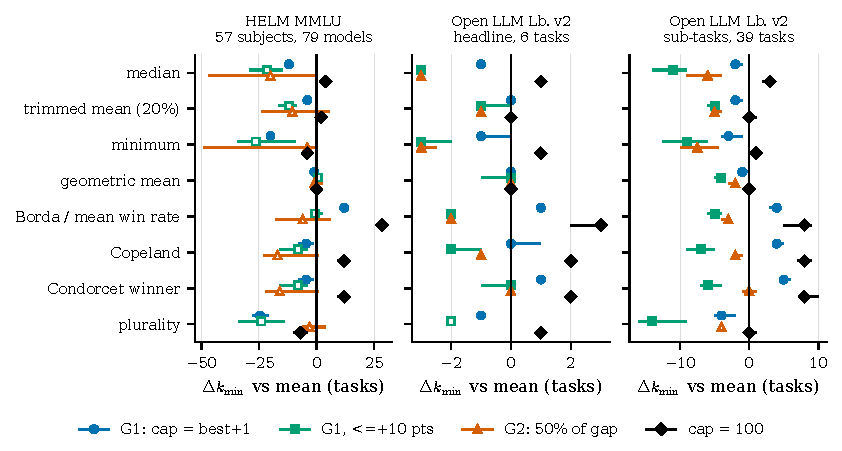
\includegraphics[width=\linewidth]{../figures/fig_c2_rules.pdf}
\caption{Median paired difference in $k_{\min}$ against the mean rule, 95\% bootstrap CI over target models, linear cost, normalised scores, targets of mean rank $\ge2$ feasible under both rules; hollow markers: fewer than 20 pairs. Open LLM Leaderboard headline targets are a rank-stratified sample. Values in Table~\ref{tab:c2} (appendix).}\label{fig:c2}
\end{figure}

\paragraph{C3: no monotone ordering along the power-mean family on HELM.}
We expected $k_{\min}$ to vary monotonically with $p$ between the minimum ($p\to-\infty$) and large $p$. Only 9--15\% of HELM targets show a monotone curve (G1: 9\%, ceiling: 15\%); the median curve is U-shaped, with the minimum cheapest and the arithmetic and neighbouring power means nearly flat (Figure~\ref{fig:c3}, appendix). On the Open LLM Leaderboard headline board, monotonicity holds for 98\% of the targets under the ceiling cap (non-increasing in $p$), but for only 29\% under G1; at the sub-task level only 15\% (G1) and 37\% (ceiling). The hypothesis fails as stated.

\paragraph{C4: feasibility falls with the initial rank only under bounded gains.}
Under G1 every target can reach first place, because a cap of ``best plus one'' always allows beating every rival on every task, so the claim cannot be tested there. Under G2 with $\gamma=0.5$ (Figure~\ref{fig:c4}), feasibility drops sharply with rank: on HELM, all of ranks 1--2 but only 75\% of ranks 3--10 (8 models) and none of ranks 11--100 can reach first place under the mean; under the minimum only 38\% of ranks 3--10. On the Open LLM Leaderboard headline board, every target in the top 100 can under the mean but only 22\% of the remaining models, and at the sub-task level (a pool of 699 models, not the full field) 60\% of the rest. Plurality is the most restrictive rule: infeasible for nearly all Open LLM Leaderboard targets and for 75\% of HELM ranks 3--10, since it requires first places. So, under bounded gains on HELM and on the six-task board, the answer to ``what investment is needed'' is ``none that suffices'' for most models outside the top ten (it is less restrictive at the sub-task level, where 58\% of the lowest-ranked sample can).
\begin{figure}[t]
\centering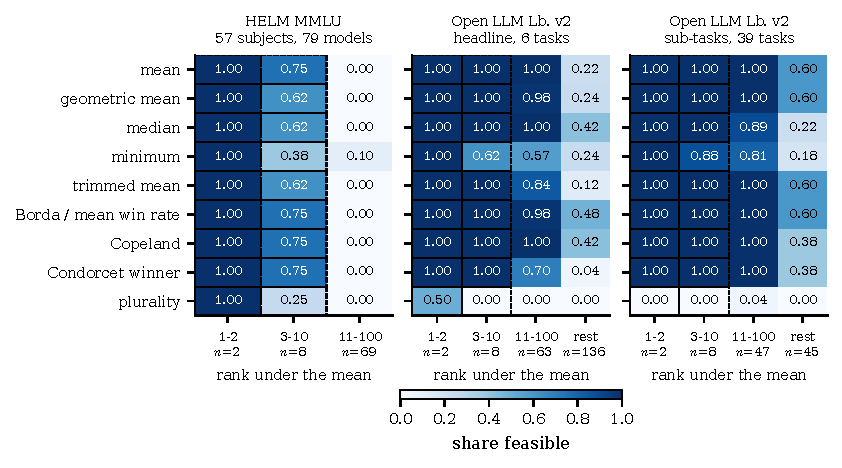
\includegraphics[width=\linewidth]{../figures/fig_c4_feasibility_G2_0.5.pdf}
\caption{Share of targets that can reach first place under gain model G2 ($\gamma=0.5$), by rank under the mean; dashed outlines: fewer than 10 targets. Open LLM Leaderboard headline targets are a rank-stratified sample.}\label{fig:c4}
\end{figure}

\paragraph{C5: the fraction of tasks that must be targeted falls with $n$.}
We hypothesised that more sub-datasets require proportionally more investment. In random task subsets of HELM (targets at mean rank 2--20 of the subset board, G1), the number of tasks needed under the mean rises from 2.3 at $n=5$ to 15 at $n=57$ while the fraction $k_{\min}/n$ falls from 0.46 to 0.26; for the minimum $k_{\min}$ stays near 2.5 (Figure~\ref{fig:c5}). On the sub-task level of the Open LLM Leaderboard $k_{\min}$ stays between one and 2.5 tasks for $n\le39$. Absolute breadth grows with $n$ but proportional breadth shrinks, so the hypothesis of proportional growth is not supported.
\begin{figure}[t]
\centering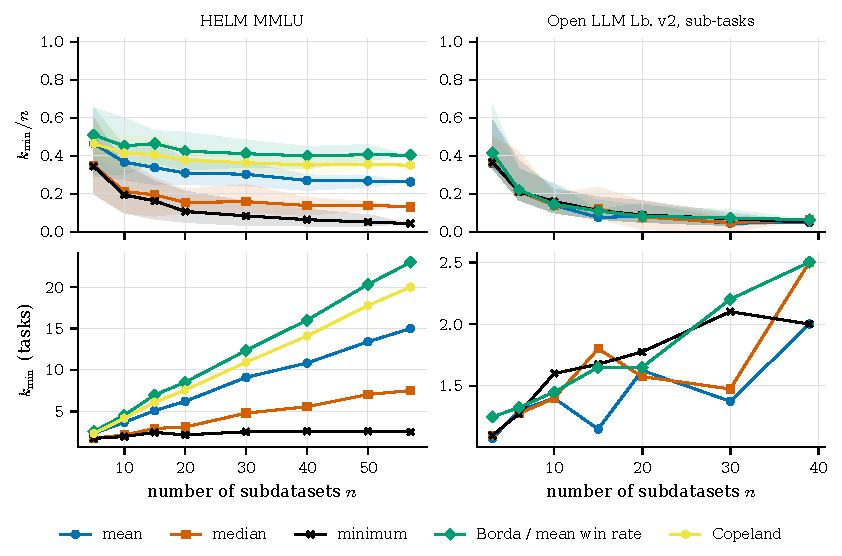
\includegraphics[width=\linewidth]{../figures/fig_c5_subsample.pdf}
\caption{Dependence of the investment on the number of sub-datasets $n$ (mean over 20 random task subsets; band: 2.5--97.5\% range of the fraction), gain model G1.}\label{fig:c5}
\end{figure}

\paragraph{C6: robustness.}
Across gain models, the Open LLM Leaderboard population (all, unflagged, without merges, official providers), raw versus normalised scores, field size (all, top 50, top 10) and granularity, the paired differences for cardinal rules are nearly identical across fields and populations, whereas those of Borda change with the field on HELM (+12 for the full field, +4 for the top-10 field), as expected for a rule that depends on the set of competitors (Table~\ref{tab:ablation}, appendix). Finer granularity increases the cost of the ordinal rules relative to the mean on the Open LLM Leaderboard (Borda $+1$ at six tasks, $+4$ at 39). Allocation baselines (Table~\ref{tab:baselines}) show that choosing the tasks matters: under the minimum and the median a random or greedy-by-headroom choice often fails where the optimal choice succeeds, whereas under the mean greedy by headroom coincides with the optimum.

\section{Discussion and Limitations}
\paragraph{What the results say.} The investment needed to take first place is determined by the rule's structure together with the gain cap. Under a cap at the best observed score, spreading modest gains over a majority of tasks (median) or over the few weak tasks (minimum) is cheaper than pooling a large total gain (mean); under a cap at the maximum score the pooled mean is cheaper than the median, the trimmed mean, Borda and Copeland, while the minimum (and plurality) stay cheaper than the mean on HELM ($-4$ and $-7$ tasks). The ordinal rules that depend on the competitors behave differently, and respond to the definition of the field. Whether a model can reach first place at all depends largely on the headroom assumption and on its initial rank.
\paragraph{Where the conclusions fail.} The conclusions fail or cannot be tested in the following conditions. (i) C4 is untestable under G1 because every target is feasible. (ii) On the Open LLM Leaderboard headline board with six tasks the differences between rules are one to three tasks and in several cells the confidence intervals include zero. (iii) The rank-based rules depend on the competitor field; the sub-task pool of 699 models is not the full field. (iv) With noise the ordering can reverse (C2 under P(first) $\ge0.9$). (v) The Condorcet-winner and Copeland results coincide in many cells and then give no independent evidence.
\paragraph{Limitations.} All results are conditional on assumed gain models; none is calibrated against real training (G4 was cut), and the cap ``best score plus one'' is a convenience, not a prediction. Spillover between tasks (training on one sub-dataset changes others) and tie-breaking variants were not run; the weighted mean, Schulze, Kemeny, maximin and the power mean at $p=+\infty$ were not studied. $G_{\min}$ for the ordinal rules and the trimmed mean is an upper bound, and the trimmed mean at more than ten tasks is solved heuristically. The Open LLM Leaderboard headline targets are a rank-stratified sample; the sub-task level uses 699 of 4{,}576 models. The data are frozen 2025 snapshots with undeclared licences; the leaderboards already contain merged and fine-tuned models that may have been trained on related data, so the observed scores are not a clean baseline. We study a single developer and not the equilibrium of several developers acting together \citep{chen2026incentives}. Evaluation noise is a Gaussian approximation of the binomial error on a subset of targets. We do not claim novelty beyond the stated formulation and its measurement: we searched the literature only on the components of the question.

\subsection*{Reproducibility statement}
Code, fetch scripts with pinned snapshot ids and checksums, seeds, commands, measured step times and a map from every table and figure to its generating script are in the supplementary material (\texttt{REPRODUCE.md}, \texttt{data/manifest.json}); the environment is CPU only.
\subsection*{Ethics statement}
The study uses only public score tables and no human subjects. The score data have no declared licence; we ship scripts and checksums but no copies. The analysis describes how leaderboard rankings could be influenced; it is not a recommendation to do so, and it does not name practices of any developer.
\subsection*{AI use statement}
This work was produced end to end by AI agents (Claude models, in an automated research workflow) with no human researcher in the loop. Required-disclosure tasks done with generative AI: designing the study and hypotheses, implementing the methods and solvers, cleaning and reformatting the data, running the analyses, interpreting the results, stating the theory and claims, and writing the paper. Recommended-disclosure tasks: writing and editing code, searching and summarising literature, producing figures, and formatting references. Statements about prior work rest on abstracts and the task's annotated reading list, not on full-text reading of every cited paper.

\bibliography{references}
\bibliographystyle{iclr2027_conference}
\appendix
\section{Additional results}
\begin{table}[h]
\caption{Median paired difference in $k_{\min}$ against the mean rule on HELM MMLU, by gain model and rule [95\% CI] (number of pairs); bold: CI above 0.}\label{tab:c2}
\centering\tiny\resizebox{\linewidth}{!}{\input{../tables/c2_helm_mmlu_headline.tex}}
\end{table}
\begin{table}[h]
\caption{Robustness grid for claim C2: median paired difference in $k_{\min}$ against the mean over feasible targets [95\% CI]; bold: CI above 0.}\label{tab:ablation}
\centering\tiny\resizebox{\linewidth}{!}{\input{../tables/ablation_c2.tex}}
\end{table}
\begin{table}[h]
\caption{Median budget $k$ needed and share of attackers that reach rank 1 within the evaluated budget, gain model G1; inf: the median attacker does not.}\label{tab:baselines}
\centering\footnotesize\input{../tables/baselines.tex}
\end{table}
\section{Literature search and independence}
The task forbids reading the earlier published paper on this question and anything citing it. We searched only for the components of the question (social choice, benchmark selection, contamination, training on the test task, the data sources) and for the titles of the starter references, and ran no forward-citation queries. One search result (a 2026 arXiv paper on perturbation analysis of Bradley--Terry leaderboards, returned for the query ``The Leaderboard Illusion Chatbot Arena'') was seen as a title and a three-line abstract snippet; it is about a different aggregation model (pairwise preferences), we stopped reading there, and we neither cite nor use it. Statements about prior work rest on abstracts and the annotated starter list, not on full-text reading of every cited paper. The analysis positions report that they encountered nothing of the prohibited kind.

\begin{figure}[h]
\centering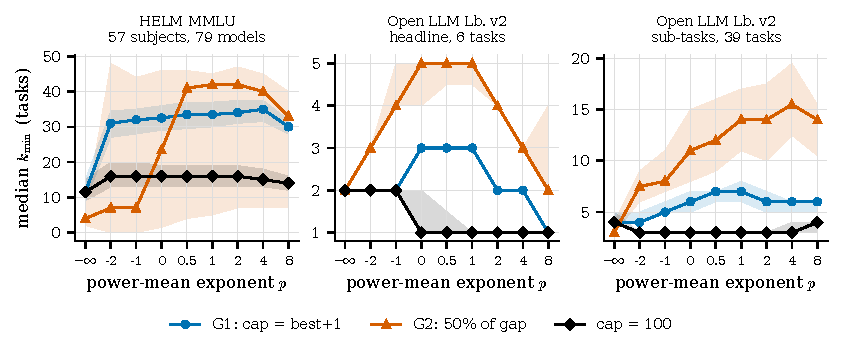
\includegraphics[width=0.9\linewidth]{../figures/fig_c3_powermean.pdf}
\caption{Median $k_{\min}$ along the power-mean family (median over attackers with mean rank $\ge2$, band: 95\% bootstrap CI over targets, linear cost).}\label{fig:c3}
\end{figure}
\end{document}
